\chapter{Design for a Single-User Recommendation Application in a DUI Environment}\label{chapter:design}

In the previous chapters, the foundations of recommender systems were introduced, as well as the basics of distributed user interfaces, their definitions, properties and the different UI distribution dimensions. In this chapter, a design for a single-user recommendation application in a distributed UI environment is proposed.

The motivation of the proposed design could be best described through the following scenario: A user of a recommendation application receives recommendations on his/her mobile device. The user of such application might be willing to migrate the recommended content to be consumed on a different device in his/her environment, as his/her mobile device's battery might be expiring, or the consumption of the recommended item would be more convenient on the other device.

The actualization of the previous scenario depicts a multi-device (and possibly multi-platform) environment, in which the flow of control (logic) and application's user interface are decoupled in a way that allows for the distribution of UI components along the different devices. In other words, the user of such system is provided with a distributed solution, which enables him/her to perform tasks on whichever device in this environment (by for example migrating the UI components between the different devices) independently of where the application is running, and of the constraints presented by the different platforms running the application.

The following section starts by describing a generic model for UI distribution of recommendation applications, following by a description of more specific scenarios relative to our distributed video recommender application.


\section{Generic Model for Recommender Systems UI Distribution}
As debriefed earlier, there are different dimensions to UI distribution. The proposed design is described through different UI distribution scenarios with respect to the following UI distribution dimensions: time, user, platform, and task. This section describes how the different distribution dimensions could alter the design decisions for a system whose UI is targeted for distribution. 

\subsection{Time: When to Distribute?}
The aspect of when the UI elements of an interactive system are to be distributed (statically at compile/load time or dynamically at runtime) is a key design decision. One way to distribute the UI is to have the distribution decisions made prior to execution, without providing the ability to alter these decisions. If the UI elements are to be distributed dynamically, for example, based on the user's needs that can only be known at runtime, a design decision to make in such case is to prepare a set of UI configurations that the system could use on loading components to adjust the UI accordingly. In such case, the system delays the final decision to which UI elements to distribute, instead of having this option preconfigured.    

\subsection{User: Who Initiates Distribution?}
In most of the scenarios, identifying whether the user or the system initiates the distribution is essential to the design. Creating a scenario in which the user detects a need for UI distribution, computes and selects an alternative scenario, requires the system to be more adaptable than the case when the system initiates the distribution. When a user initiates the UI distribution, they could select components to be displayed on the systems' platforms. Later, they could also reside to the possibility of restoring the UI to its original state, or keep the new configuration saved for later use. Alternatively, the system designer could detect a need for distribution and configure the system to initiate the UI distribution on, for example, carrying out specific tasks, or if the system is loaded with a specific configuration.    
 
\subsection{Platform: Where to Distribute?}
It can be fairly assumed that a distributed scenario is probably going to involve different platform. In every distributed scenario, on which platform the UI components are decided (by system or user, dynamically or statically) to reside would alter how the UI needs to be adjusted to best fit the new platform. For example, allowing a UI to be transferred between a limited display of a PDA and a larger display such as a tabletop would require adjustment for how the different UI components are to be adjusted to fit the limitations of each platform.   

\subsection{Task: What to Distribute?} 
One prespective to look at the distribution of recommender system is to identify the recommendation tasks that could be distributed. For a system to be distributed, one or many tasks should be considered to be carried out simultaneously or not in a distributed way. A task could be distributed into several subtasks to be carried out by one user, but on different platforms, in the same environment, over time. 
For the proposed distributed recommender system design, the following tasks are considered for distribution: presentation of recommended items, item consumption, recommended content filtering, and recommended content rating.\\ 
UI components constituting the interactive systems through which a user could undertake such tasks could be thought of as the unit of UI distribution. In the distribution of such tasks, full or part of the UI can be transferred among platforms and devices through a simple user action, such as a gesture. For user input and interaction with the system, the use of gesture, such as panning and swiping, is considered to reduce cognitive overhead [cite]. The decomposability of the system components enables one or more of the distributed UI elements to be executed independently without losing their functionality. It is also important to ensure the consistency of performing the different distributed actions; i.e. to ensure that a distributed action (for example phase of recommendation) is supported on the different platforms. Such actions can be carried out in various ways, hence, increasing the flexibility of the system. \\

\subsection{Migrating Item Consumption}
One of the main distribution scenarios to consider is the distribution of the task of recommended items consumption. Unlike the regular scenario, where the user of a recommender system is presented with the recommended items and is able to select and consume an item on the same device, a distributed alternative would be to present the recommended content on one device while giving the user the ability to consume the content on the other device. As shown in figure \ref{fig:figure31}, this scenarios could be triggered by the user performing a gesture on one of the items presented on the presentation node (i.e. the node that would contain the presentation of the recommended content). The item consumption task is now migrated to be carried out on the other device/platform. 
\begin{figure}[h]
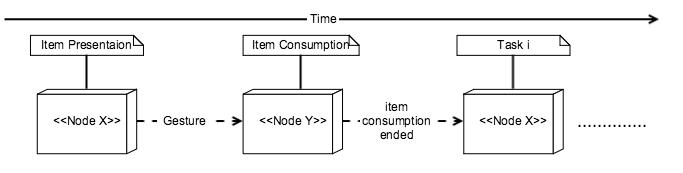
\includegraphics[width=0.9\textwidth, inner, center]{generic1}
\caption{Migrating Item Consumption from Presentation Node to Consumption Node.}
\label{fig:figure31}
\end{figure}

\subsection{Performing Parallel Activities}
\begin{figure}[h]
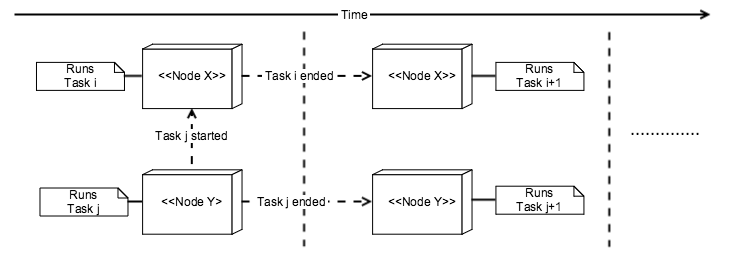
\includegraphics[width=0.9\textwidth, inner, center]{generic2}
\caption{Caption}
\label{fig:figure32}
\end{figure}
In a distributed environment, presenting the user with different platforms through which the user could perform tasks simultaneously could be leverage to perform parallel activities. In this case the distribution is achieved through distributing different interface components to be executed asynchronously (distribution in time). In contrast to the non-distributed scenario in which the user usually can not perform UI related tasks in parallel (asynchronously), but would usually wait for a UI task to be done before he/she could start the next (synchronously). Figure \ref{fig:figure32} is showing how a task could start running on a given node in the distributed environment, denoted here by task j on node Y, which triggers task i to start on node X. In this case, tasks are run in parallel and the user can perform these activities independently from each other and simultaneously. This is a case of distribution in time. After the tasks end on their given node, execution of proceeding tasks could be carried out also in a distributed manner. 
\subsection{Overview And Detail Presentations}
In a distributed environment with multiple displays, LD-SD modes are used to show different versions of the presented content to the user. There is always a concern on using different modes of what to choose to present to the user on which display/mode and what would be the basis for this choice. There is also the question of how to present the content differently on each mode based on its capabilities. Figure \ref{fig:figure33} suggests presenting a detailed presentation  of content on the SD on which the user could get all available detailed information of the provided content (for example in a form of a detailed list), while on the LD, the user could be presented with an overview of the same content (for example, in the form of picture icons with titles presented with in different sizes). Selecting an item on either mode later could lead to the execution of a proceeding task on either platform such as item consumption or viewing more information for the item.      

\begin{figure}[h!]
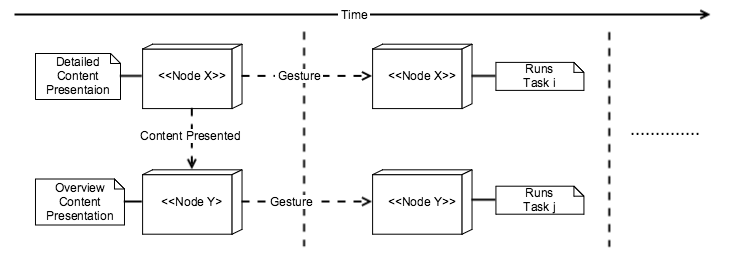
\includegraphics[width=0.9\textwidth, inner, center]{generic3}
\caption{Overview-Detail Presenations}
\label{fig:figure33}
\end{figure}


\subsection{Content Filtering}
As the user is presented with a wide array of recommended content, he/she might be willing to filter his/her choice of what to consume of this content. On a multi-device/platform environment, the filtering task could be distributed along the different nodes of the system. As shown in figure \ref{fig:figure34}, the user could initiate a gesture on items on node X to be transferred/redirected to node Y. By the end of this process, the user ends up with a presentation of all the selected/filtered items on node Y. The user could next select one of these items to view more details. This is an example of synchronous task distribution along different platforms.
  
\begin{figure}[h!]
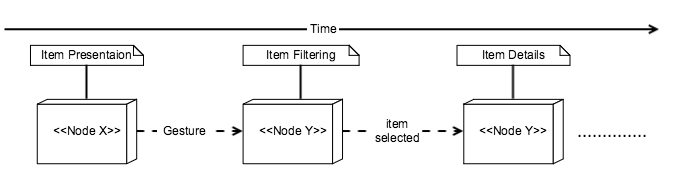
\includegraphics[width=0.9\textwidth, inner, center]{generic4}
\caption{Recommended Content Filtering}
\label{fig:figure34}
\end{figure}

\subsection{Content Redirection}
Content (output) redirection is a key feature in a multi-device environment [cite]. It is argued to be more important in case of multi-user systems, however, it could still be leveraged for single-user scenarios. Item consumption redirection is considered one special case of content redirection. Other examples would be redirecting recommended content details to be presented between SD and LD displays. Figure \ref{fig:figure35} shows how node X presents the recommended content, while on performing a gesture on any of the items, this content could be transferred/redirected to be presented on node Y. This usually means the distribution of UI components representing this content is what enables the redirection of content seamlessly between the two presentation nodes. The user could possibly then proceed with item consumption on the same node or on a different node.   
\begin{figure}[h!]
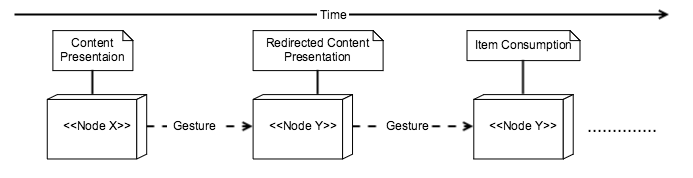
\includegraphics[width=0.9\textwidth, inner, center]{generic5}
\caption{Content Redirection}
\label{fig:figure35}
\end{figure}
\section{Design for a Single-User Video Recommender System in a Distributed UI Environment}
The proposed design is for a single-user, multi-device video cast recommendation application, in which the user interface and recommendation subtasks are distributed along the devices. The goal of the design is to leverage the capabilities of the distributed UI environment in order to find a new way to present the recommendation tasks and results to the user. In this section, we show how the recommendation tasks such as presenting the recommended items, item consumption, item rating, and others could be done in a distributed fashion. Our design is mainly targeted at benefiting from both platforms to make the post-recommendation phase of such system more efficient and more user-centric.
\subsection{Distribute for Whom?: UI Distribution In a Single-User System}

Our goal is the UI distribution of a single-user recommender system. The case for UI distribution of group recommenders in a multi-user environments has been made by a number of studies [cite]. The group recommendation involve multiple users with multiple devices. And since the main goal of a group recommendation is to reach consensus about a recommendation, distributed UI components that could be shared among the group members to reach this consensus is needed.

Less research have been made to make a case for the use of UI distribution of for single-user recommender systems. In such system, since a single user is involved in the process, and the consensus activity does not exist, it could be more challenging to think of what the distribution could be useful for in a single-user scenario. The main question on designing for such a system is to answer the question of why a single user would need a distributed environment; one with multiple devices and platforms. Why and if the action of recommendation for a single user with its various phases could be carried out on multiple devices/platforms, and whether the overhead(refer to the overhead described in earlier chapter) of distribution such a system is of an added value. The main challenge would be the introduction of a distribution mechanism for this system in such a way that does not hinder the process, and that would actually serve it. Also, the distribution should be done in such a way that does not introduce an overhead of shifting the user's attention from one platform/device to the other. 

\subsection{Platforms and Environment}
\begin{figure}[h!]
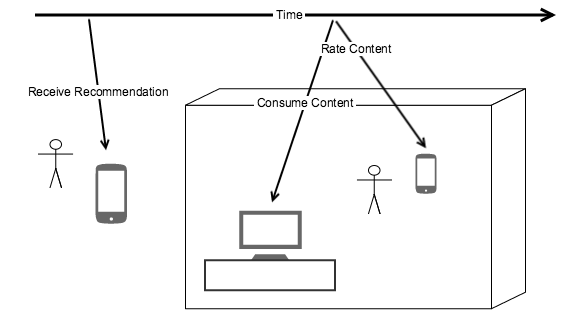
\includegraphics[width=0.6\textwidth, inner, center]{env}
\caption{Overall view of the system's environment}
\label{fig:figure311}
\end{figure}
To address some of the challenges mentioned in the previous section about designing for single-user in a distributed UI environment, we started by thinking of a scenario in which the user would be in need of, or would prefer to, use multi-devices to carry out the recommendation tasks. This lead us to think of a scenario that would start in a mobile environment. Figure \ref{fig:figure311} describes how the user receives recommendation for a new video cast on his/her mobile device while for example in commute. Since video content is usually lengthy and would be better viewed on a larger display than the limited space available on a mobile device display, the consumption of this content is thought to be better migrated to a large display device. The user could then migrate the consumption of this content to the LD once he/she reaches the environment that contains the LD (office, home, etc..). The application would then continue to operate in SD-LD mode; i.e. distributed among the mobile device (SD) and an LD, such that the user would be able to watch the video on the LD. In the following section, the distribution of video consumption as well as other recommendation subtasks are described.          
\subsection{Recommendation Tasks in a Distributed UI Environment}
In this section, the concept behind the distribution of pre and post recommendation tasks is provided. The reason for which tasks or UI components are selected to be displayed on which display, as well as the description of other distribution dimensions, are given.
\subsubsection{User Profile Creation}
The pre-recommendation phase usually starts by the elicitation of a user profile. Creating a profile usually involves filling out information forms, and likely rating some prototype items or entering preferences. This step would differ from one system to the other. For the video recommender, this involves asking the user directly to enter basic information and to rate a list of topics and interests to give a background about the user's preferences. 
The assumption in this step is that filling out textual forms as well as rating would better be performed on the handheld device than a larger display. The user is assumed to have more control over input for smaller devices. Therefore, this task starts at in the SD. As shown in figure, after the user finishes the profile creation step on the SD, the recommended content is then displayed on both SD and LD displays.
\begin{figure}[h!]
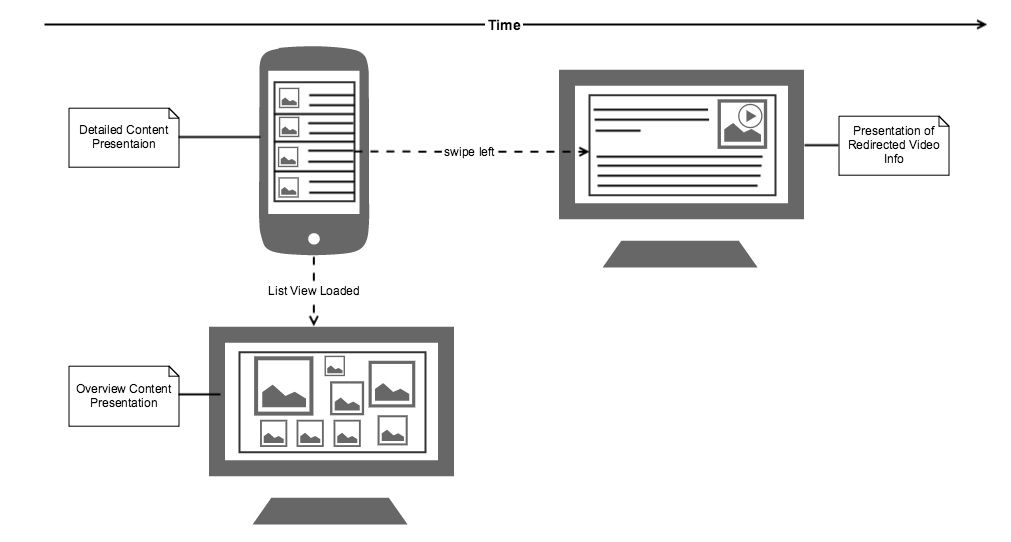
\includegraphics[width=0.85\textwidth, inner, center]{presentation-detail}
\caption{Presentation of Recommendation Results in LD-SD Modes.}
\label{fig:figure38}
\end{figure} 
\subsubsection{Presentation of Recommendation Results}
The presentation of recommended video casts is shown in parallel on the SD and LD, however, in different formats. We propose to present the recommended content at a different level of granularity for each platform; fine granularity is offered on the mobile device while coarse level of presentation is provided on the LD. As shown in figure \ref{fig:figure38}, for the mobile device, a detailed list of all the recommended videos, together with detailed information about the video, are shown in tabular form with different categorization. On the LD, an overview presentation is shown for the recommended items that scored the highest for the user without details, however shown in different sizes to indicate the recommendation score.
This way, we provide the user with alternative ways to view the content. At a glance, he/she could get an overview of the provided content with a graphical indicator for the recommendation score. Then, if more details is needed, the mobile device would provide more a detailed information about the video content. This concept UI distribution is what comes to be known as overview-detail coupling [cite].\\ 
For presenting the user with detailed information about the recommended videos, the recommendation list offers a link to a detailed information page on the mobile device in a master-detail fashion. As the user clicks on the item in the list, the user enters the detailed information page on the mobile device. Alternatively, as shown in figure \ref{fig:figure38} content redirection is also possible for viewing such information on the LD. Also by applying a simple swipe-right gesture on any of the video items in on the SD list, the video details content will be redirected to be displayed in parallel on the LD.   
    
\subsubsection{Recommended Item Consumption}
Playing the recommended videos is done as depicted by figure \ref{fig:figure36}. On the video details page, the user performs a pan gesture on the video image,  which then triggers the migration of the video consumption from the mobile device to the LD. The video player automatically stars on the LD, providing the user with all controls for the video playback.  
\begin{figure}[h!]
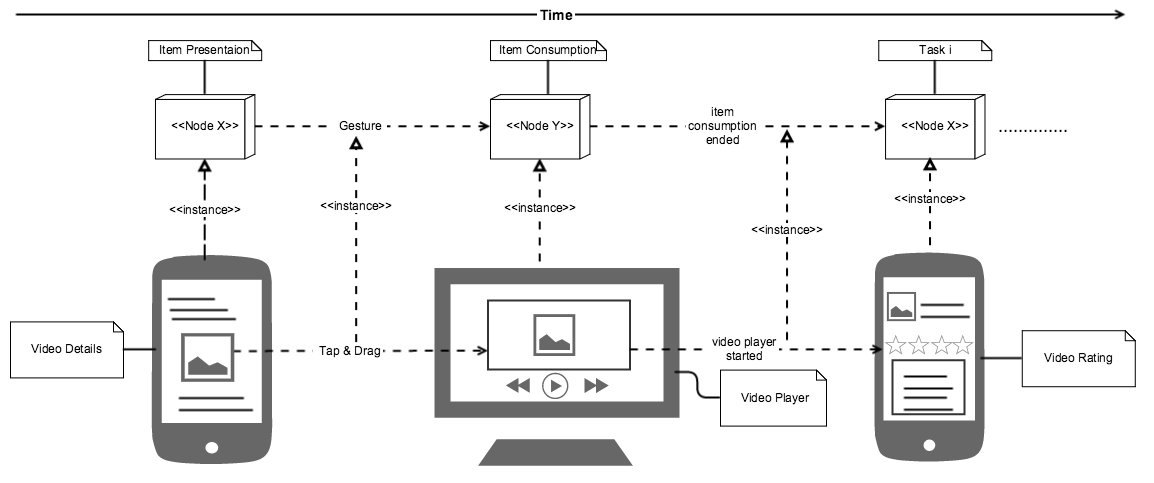
\includegraphics[width=0.9\textwidth, inner, center]{playrate}
\caption{Recommended Items Consumption.}
\label{fig:figure36}
\end{figure}
\subsubsection{Rating of Recommended Items}
There are two different proposed options for the rating task. The first option is distributed in time; i.e. done in parallel with the video playback. As shown in figure \ref{fig:figure36}, after the video playback starts automatically on the LD as described in the previous section, the LD triggers the mobile device to display the rating page for the user on the SD. Hence, the two tasks could be carried out simultaneously by the user.
Alternatively, the user could also be triggered to enter the rating on the mobile device after the video has ended playing or if stopped by the user on the LD. In such case, there is no parallelization of the tasks, however there is still synchronisation between the tasks that are carried out synchronously on the different platforms.\\
The rating, similar to the user profile creation, include user input such as indication of likes or entering textual comments and reviews, which is also believed to be best done on a mobile device with a better controlled input, for the user's convenience.  

\subsubsection{Filtering Recommended Items}
The filtering for the recommended items, although not a main task in recommendation, is believed to add to the value of the system in the proposed distributed UI environment. It is one of the tasks that leverages from the availability of the different platforms for the benefit of the user's experience. As shown in figure \ref{fig:figure39}, the filtering is done by performing a left swipe gesture on the video item in the list view on the mobile device.
\begin{figure}[h!]
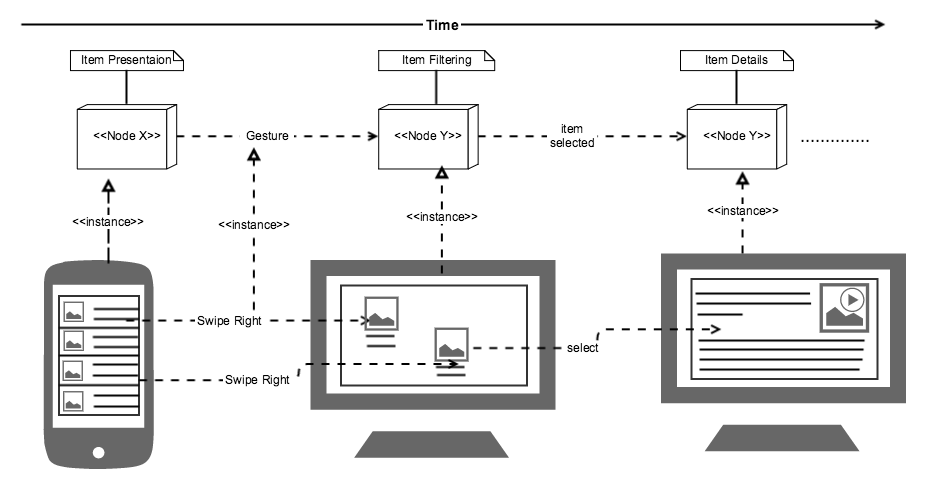
\includegraphics[width=0.85\textwidth, inner, center]{filtering}
\caption{Filtering of Recommended Items.}
\label{fig:figure39}
\end{figure}
This gesture redirects the content of the video to the LD. The display of the content on the LD is also done in a overview-detail coupling manner as described in earlier section. After the user is done filtering (redirecting selected content from SD to LD), LD will contain all the selected items displayed in an overview fashion. More details could be access through the SD or by also clicking on the item on the LD.  

\subsection{Transferring Recommendation Lists}
-Example of distribution initiated by user... (basically any type of content redirection)\\
-Select which components within a view (details view) are to be distributed.\\
-Readjust to old view after that
-Save as a configuration
-Rating: in parallel or after player?

\subsection{Pre-Configuring the System}
Meta UI. Time distribution. Enables system to load components differently at runtime. Select a configuration. Selecting which views to show on which platform.  

